\documentclass{article}

\usepackage{graphicx}
\usepackage{geometry}
 \geometry{
 a4paper,
 total={170mm,257mm},
 left=20mm,
 top=20mm,
 }

\begin{document}
\section*{Design Documentation (OpenID Connect Doctor)}
\subsection*{Architecture}
The OpenID Connect Doctor consists out of a frontend and a backend. The frontend consits out of multiple views, which are shown to the users. Each view represents one part of the frontend and commuicates with one module in the backend. The backend of the application consits out of mutliple modules, which provide the logic for the application. Every module is stored in a separated folder and consits of some or all of the following components. 
\begin{itemize}
    \item Service containing the logic. (naming-convention: *.service.ts)
    \item Spec containing the unit test. (naming-convention: *.spec.ts)
    \item Controller handling the comunication with the frontend, handling user-input and controlling what is displayed to the user. (naming-convention: *.module.ts)
    \item Data Tranfer Objects used to transfer data between the frontend and the backend. (*.dto.ts)
\end{itemize} 
The diagram below displays the general structure of the OpenID Connect Doctor.

\begin{figure}[h]
    \centering
    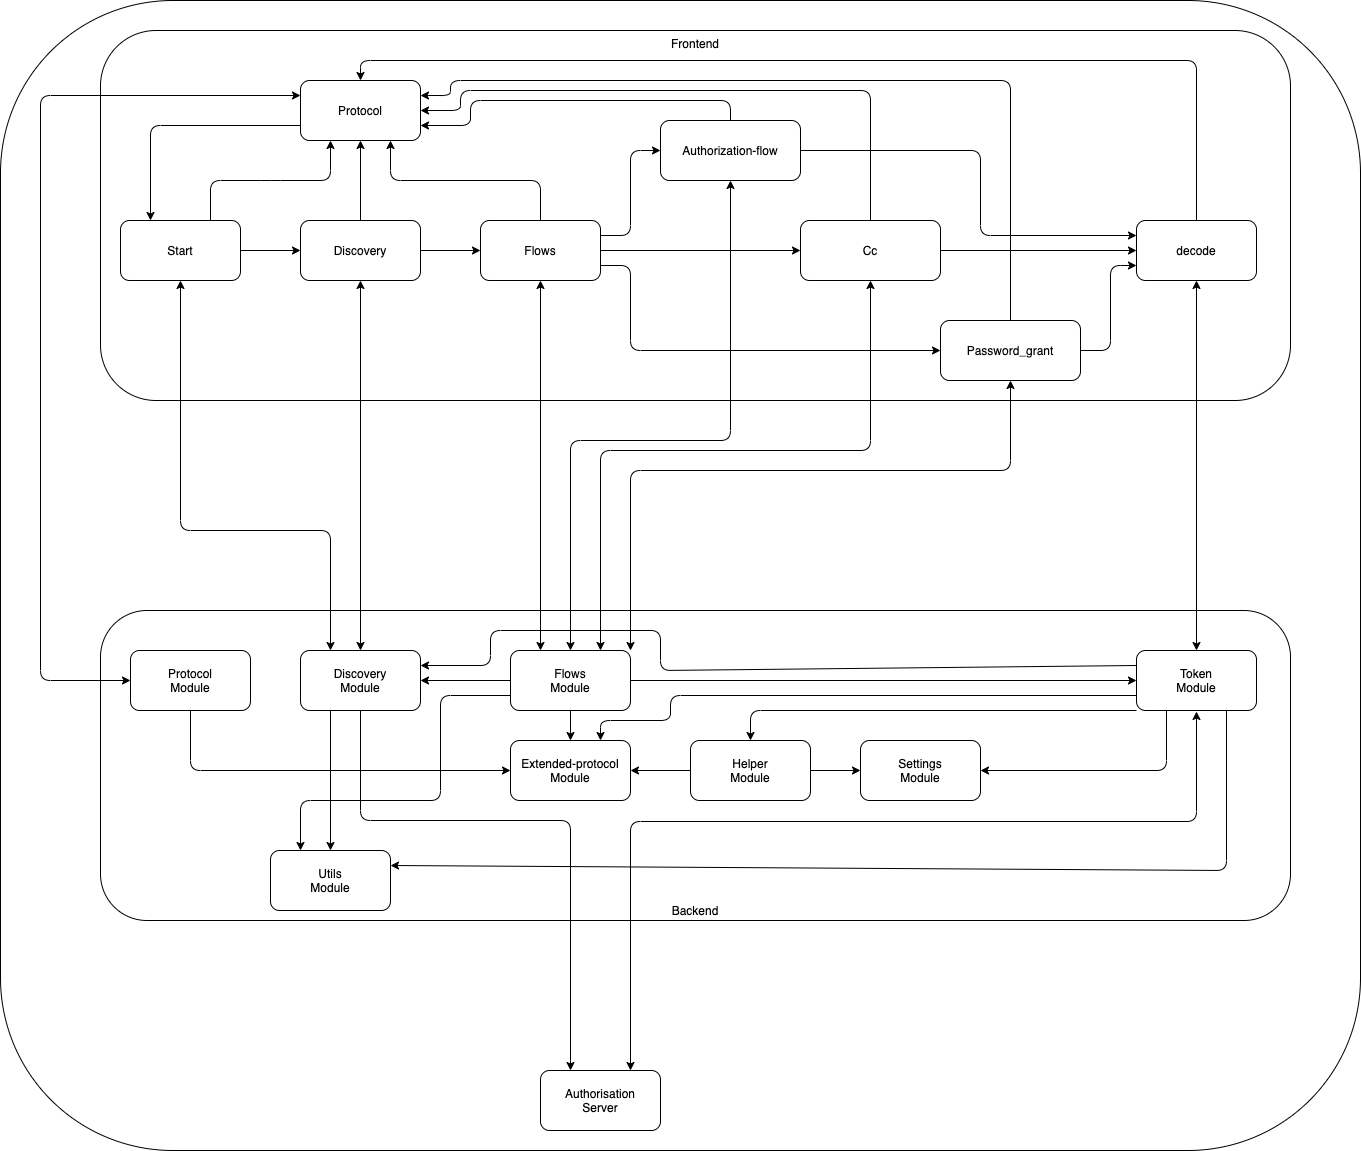
\includegraphics[width=\textwidth]{design}
    \caption{OpenID Connect Doctor Desgin}
\end{figure}

\end{document}